\documentclass[10pt]{article}
\usepackage[utf8]{inputenc}
\usepackage{tikz}
\usetikzlibrary{shapes.geometric,arrows}
\usetikzlibrary{positioning,shadows}
\usepackage{relsize}
\usepackage{booktabs}
\usepackage{graphicx}
\usepackage{adjustbox}
\usepackage{setspace}
\usepackage{graphbox}
\usepackage{calc}
\usepackage{tipa}
\usepackage{layouts}
\usepackage[papersize={182mm,185mm},margin=1mm]{geometry}

\begin{document}
\sffamily 
\scriptsize % 7pt sans-serif

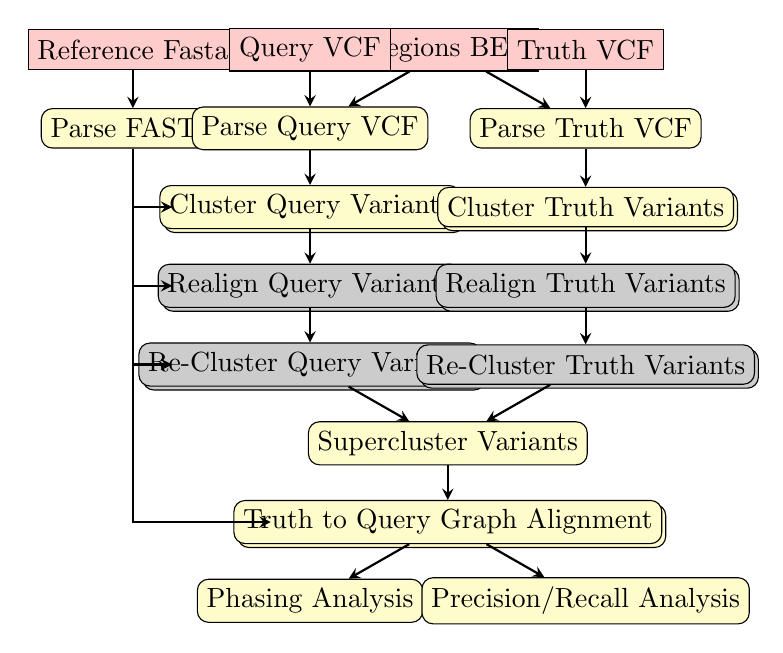
\begin{tikzpicture}[scale=0.5]
% define box types
\tikzstyle{mystep}=[draw,rectangle, rounded corners, fill=yellow!20,
    minimum width=15mm, minimum height=5mm]
\tikzstyle{optstep}=[draw,rectangle, rounded corners, fill=black!20,
    minimum width=15mm, minimum height=5mm]
\tikzstyle{mystep2}=[draw,rectangle, rounded corners, fill=yellow!20,
    minimum width=15mm, minimum height=5mm, 
    copy shadow={draw, shadow xshift=0.5mm, shadow yshift=-0.5mm}]
\tikzstyle{optstep2}=[draw,rectangle, rounded corners, fill=black!20,
    minimum width=15mm, minimum height=5mm, 
    copy shadow={draw, shadow xshift=0.5mm, shadow yshift=-0.5mm}]
\tikzstyle{mystep4}=[draw,rectangle, rounded corners, fill=yellow!20,
    minimum width=15mm, minimum height=5mm, 
    copy shadow={draw, shadow xshift=1.5mm, shadow yshift=-1.5mm},
    copy shadow={draw, shadow xshift=1mm, shadow yshift=-1mm},
    copy shadow={draw, shadow xshift=0.5mm, shadow yshift=-0.5mm}]
\tikzstyle{optstep6}=[draw,rectangle, rounded corners, fill=black!20,
    minimum width=15mm, minimum height=5mm, 
    copy shadow={draw, shadow xshift=2.5mm, shadow yshift=-2.5mm},
    copy shadow={draw, shadow xshift=2mm, shadow yshift=-2mm},
    copy shadow={draw, shadow xshift=1.5mm, shadow yshift=-1.5mm},
    copy shadow={draw, shadow xshift=1mm, shadow yshift=-1mm},
    copy shadow={draw, shadow xshift=0.5mm, shadow yshift=-0.5mm}]
\tikzstyle{input}=[draw, rectangle, fill=red!20, minimum width=15mm, minimum height=5mm, aspect=3]
\tikzstyle{a}=[thick,->,>=stealth]
% inputs
\node[input] (fasta) at (0,0) {Reference Fasta};
\node[input] (bed) at (8,0) {Regions BED};
\node[input] (query) at (4.5,0) {Query VCF};
\node[input] (truth) at (11.5,0) {Truth VCF};
% steps
\node[mystep] (pfasta) at (0,-2) {Parse FASTA};
\node[mystep] (pquery) at (4.5, -2) {Parse Query VCF};
\node[mystep2] (cquery) at (4.5,-4) {Cluster Query Variants};
\node[optstep2] (rquery) at (4.5,-6) {Realign Query Variants};
\node[optstep2] (c2query) at (4.5,-8) {Re-Cluster Query Variants};
\node[mystep] (ptruth) at (11.5,-2) {Parse Truth VCF};
\node[mystep2] (ctruth) at (11.5,-4) {Cluster Truth Variants};
\node[optstep2] (rtruth) at (11.5,-6) {Realign Truth Variants};
\node[optstep2] (c2truth) at (11.5,-8) {Re-Cluster Truth Variants};
\node[mystep] (sc) at (8,-10) {Supercluster Variants};
\node[mystep2] (align) at (8, -12) {Truth to Query Graph Alignment};
\node[mystep] (phase) at (4.5, -14) {Phasing Analysis};
\node[mystep] (summary) at (11.5, -14) {Precision/Recall Analysis};
% first layer
\draw[a] (fasta) -- (pfasta);
\draw[a] (pfasta) -- (0, -4) -- (1, -4);
\draw[a] (pfasta) -- (0, -6) -- (1, -6);
\draw[a] (pfasta) -- (0, -8) -- (1, -8);
\draw[a] (pfasta) -- (0, -12) -- (3.5, -12);
\draw[a] (query) -- (pquery);
\draw[a] (truth) -- (ptruth);
\draw[a] (bed) -- (pquery);
\draw[a] (bed) -- (ptruth);
\draw[a] (pquery) -- (cquery);
\draw[a] (cquery) -- (rquery);
\draw[a] (rquery) -- (c2query);
\draw[a] (ptruth) -- (ctruth);
\draw[a] (ctruth) -- (rtruth);
\draw[a] (rtruth) -- (c2truth);
\draw[a] (c2truth) -- (sc);
\draw[a] (c2query) -- (sc);
\draw[a] (sc) -- (align);
\draw[a] (align) -- (phase);
\draw[a] (align) -- (summary);
\end{tikzpicture}

\end{document}
